% =============================================================================
%  Project 9: Quantifying the Stall Penalty of a Shared Memory Port
%  in a Single-Cycle CPU
%  IEEE conference paper (IEEEtran, two-column).
%  Compile with pdfLaTeX or Tectonic. Every figure is drawn in native TikZ, so
%  the paper has no external image dependency.
% =============================================================================
\documentclass[conference]{IEEEtran}
\IEEEoverridecommandlockouts

\usepackage[T1]{fontenc}
\usepackage[utf8]{inputenc}
\usepackage{amsmath,amssymb,amsthm}
\usepackage{mathtools}
\usepackage{graphicx}
\graphicspath{{./}{diagrams/}}
\usepackage{booktabs}
\usepackage{array}
\usepackage{tabularx}
\usepackage[table]{xcolor}
\usepackage[caption=false,font=footnotesize]{subfig}
\usepackage{algorithm}
\usepackage{algpseudocode}
\usepackage{listings}
\usepackage{tikz}
\usetikzlibrary{positioning,arrows.meta,calc,automata}
\usepackage{textcomp}
\usepackage{url}
\usepackage[hidelinks]{hyperref}
\usepackage[capitalise,nameinlink]{cleveref}

% ----------------------------------------------------------------------------
%  Theorem environments
% ----------------------------------------------------------------------------
\newtheorem{definition}{Definition}
\newtheorem{proposition}{Proposition}
\newtheorem{corollary}{Corollary}
\crefname{definition}{Definition}{Definitions}
\crefname{proposition}{Proposition}{Propositions}
\crefname{corollary}{Corollary}{Corollaries}
\crefname{lstlisting}{Listing}{Listings}
\crefname{algorithm}{Algorithm}{Algorithms}

% ----------------------------------------------------------------------------
%  Palette
% ----------------------------------------------------------------------------
\definecolor{pnink}{HTML}{14213D}
\definecolor{pnslate}{HTML}{5A6B7B}
\definecolor{pnblue}{HTML}{1D6FE0}
\definecolor{pngreen}{HTML}{1E8E5A}
\definecolor{pnred}{HTML}{D1453B}
\definecolor{pnamber}{HTML}{B8860B}
\definecolor{pnbg}{HTML}{F0F2F5}

\lstset{
  language=Verilog, basicstyle=\ttfamily\scriptsize,
  keywordstyle=\color{pnblue}\bfseries, commentstyle=\color{pnslate}\itshape,
  backgroundcolor=\color{pnbg}, frame=none, xleftmargin=2pt,
  columns=fullflexible, keepspaces=true, showstringspaces=false,
  aboveskip=4pt, belowskip=2pt, captionpos=t,
  morekeywords={assign,wire,reg,always,posedge,localparam,parameter}
}

% ----------------------------------------------------------------------------
%  Macros
% ----------------------------------------------------------------------------
\newcommand{\NLS}{N_{\mathrm{LS}}}
\newcommand{\Tharv}{T_{\mathrm{H}}}
\newcommand{\Tshr}{T_{\mathrm{S}}}
\newcommand{\sig}[1]{\texttt{\detokenize{#1}}}
\newcommand{\safeimage}[2]{%
  \IfFileExists{#2}{\includegraphics[width=#1]{#2}}{%
    \fbox{\parbox[c][2.4cm][c]{0.95#1}{\centering\footnotesize
      Image \texttt{\detokenize{#2}} not found: place it next to \texttt{docs/report.tex}.}}}}

% Float-only pages start at the top instead of being vertically centred.
\makeatletter
\setlength{\@fptop}{0pt}
\setlength{\@dblfptop}{0pt}
\setlength{\@dblfpsep}{12pt}
\makeatother
\renewcommand{\dbltopfraction}{0.9}
\renewcommand{\topfraction}{0.9}
\renewcommand{\textfraction}{0.07}

\begin{document}

\title{Project 9: Quantifying the Stall Penalty of a Shared\\Memory Port in a Single-Cycle CPU}

\author{
\IEEEauthorblockN{Aryan Vibhuti, Saswataduity Bhuin, Debasish Karan, Aryu Rao, and Sayan Bhattacharya}
\IEEEauthorblockA{Computer Architecture, Semester-5 MCA Project~9: Instruction and Data Memory Hierarchy\\
Source code and artifacts: \url{https://github.com/3ncryptor/Sem-05-MCA-Project}}
}

\maketitle

% =============================================================================
\begin{abstract}
A processor that executes one instruction per cycle must fetch that instruction and, when the
instruction is a load or a store, access its operand within the same cycle. Whether the fetch and
the data access can proceed together depends entirely on whether they share one memory port. This
paper implements a 16-bit, four-instruction (\textsc{halt}, \textsc{add}, \textsc{load},
\textsc{store}), single-cycle processor once in Verilog-2001 and connects it, without any change to
the processor itself, to two memory systems that differ only in how the \texttt{stall} input is
driven: a Harvard system with independent instruction and data memories, and a shared,
single-ported (von~Neumann) system arbitrated by a two-phase controller. The controller determines
whether to stall from the opcode bits of the word it has just fetched rather than from the
processor's own read/write-enable outputs, which removes a combinational loop present in the more
direct implementation. We derive $\Tshr = \Tharv + \NLS$, giving a cycles-per-instruction of $1+f$
for the shared system, where $f$ is the fraction of executed instructions that touch data memory.
Three self-checking programs and a fault-injection test (replacing the adder with a subtractor)
validate the testbenches, and we additionally re-ran the full Icarus~Verilog~13.0 simulation suite
ourselves for this paper, instrumenting the shared controller to record its memory-port address on
every cycle. All six Harvard/shared $\times$ three-program configurations pass, and the recorded
address sequence for the representative program matches the model exactly: 5~cycles on Harvard
versus 8~on the shared system, with the extra 3~cycles landing precisely on its 3~loads/stores.
\end{abstract}

\begin{IEEEkeywords}
Harvard architecture, von~Neumann architecture, structural hazard, memory-mapped I/O, single-cycle
processor, register-transfer level, Verilog, Icarus Verilog.
\end{IEEEkeywords}

% =============================================================================
\section{Introduction}
% =============================================================================

Every stored-program processor retrieves two kinds of words from memory: the instructions it
executes and the operands those instructions read or write. If both streams are served by a single
memory with a single port, an instruction fetch and a data access cannot complete in the same
cycle; one of them must wait. This is the classical \emph{von~Neumann bottleneck}. The Harvard
organization avoids the conflict by construction, giving instructions and data independent storage
and independent address/data lines, at the cost of a fixed hardware split between code space and
data space.

The qualitative claim --- ``Harvard is faster because it overlaps fetch and data access'' --- is
easy to state and easy to believe without ever being measured. This project's objective is to make
the claim concrete: implement a simplified Harvard memory organization, connect it to a processor
simple enough that every signal can be inspected, execute programs that exercise both instruction
fetches and data accesses, and compare the result, cycle for cycle, with a shared-memory
organization built from the \emph{same} processor. Everything except the memory organization is
held fixed between the two systems --- the processor, the three test programs, and the data
address map --- so that any difference in cycle count can be attributed to the memory organization
alone.

This paper makes four contributions:
\begin{enumerate}
  \item A single-cycle processor with one stall input, instantiated unchanged inside a Harvard
        top-level module and inside a shared-memory top-level module
        (\cref{sec:design}).
  \item A two-phase shared-memory controller that derives its stall decision from the opcode bits
        of the word just read from memory, which avoids a combinational loop that the more direct
        design (stalling on the processor's own \sig{d_re}/\sig{d_we}) would create
        (\cref{sec:controller}).
  \item A closed-form cycle model, $\Tshr = \Tharv + \NLS$, together with a throughput bound
        $\mathrm{IPC}_{\mathrm{S}} \le 1/(1+f)$, derived from the controller's behaviour rather
        than assumed (\cref{sec:model}).
  \item An independently re-run verification pass for this paper: beyond the repository's own
        self-checking testbenches, we instrumented the shared controller to print its memory-port
        address every cycle and confirm, address by address, that the stall mechanism behaves as
        the model predicts (\cref{sec:results}).
\end{enumerate}

\Cref{sec:background} reviews the background, \cref{sec:design} presents the design, the model, and
the experimental setup, \cref{sec:results} presents and discusses the results, and
\cref{sec:conclusion} concludes.

% =============================================================================
\section{Background and Related Work}
\label{sec:background}
% =============================================================================

\subsection{Von~Neumann and Harvard Organizations}
In the von~Neumann machine, instructions and data occupy one address space and are reached through
one memory port. This makes the split between code and data a software decision and lets a running
program be inspected or modified as data, but it means an instruction fetch and a data access
contend for the same port. The Harvard organization, named after the Harvard Mark~I, instead gives
instructions and data separate memories with separate address and data lines, so a fetch and a data
access can proceed in the same cycle, and a store instruction can never overwrite the program
because the instruction store has no write port. \Cref{tab:orgs} summarizes the properties this
project actually builds and measures.

\begin{table}[t]
\centering
\caption{The Two Organizations as Built in This Project}
\label{tab:orgs}
\footnotesize
\begin{tabularx}{\columnwidth}{@{}l X X@{}}
\toprule
 & \textbf{Shared (von~Neumann)} & \textbf{Harvard} \\
\midrule
Storage & One 64-word array, code and data & Two independent 64-word arrays \\
Port(s) & One address/data port, 1 access/cycle & Two ports, 2 accesses/cycle \\
Load/store cost & Fetch cycle, then data cycle & Fetch and data, same cycle \\
Code integrity & A store to 0x00--0x0F could alter code & Instruction memory has no write port \\
\bottomrule
\end{tabularx}
\end{table}

\subsection{Structural Hazards}
A structural hazard arises when two operations in the same cycle require the same piece of
hardware. A single memory port needed by both an instruction fetch and a data access is the
textbook example, and it is resolved either by stalling one of the two operations or by
duplicating the resource, which is exactly what separating instruction and data memory does.
Commercial processors typically do both: separate level-one instruction and data caches (a
Harvard front end) sit in front of one shared main memory (a von~Neumann back end), an arrangement
usually called the \emph{modified Harvard} architecture.

\subsection{Why the Hazard Needs a Single-Cycle Processor to Be Visible}
The project's own design notes record the reasoning behind this choice explicitly: a multi-cycle
processor already spends separate cycles on fetch, decode, execute, and memory access, so a shared
memory could serve the fetch in one of those cycles and the data access in another, and the two
organizations would take the same number of cycles --- there would be nothing to compare. A
single-cycle processor needs its operand in the \emph{same} cycle as its fetch, so a single
shared port cannot supply both, and the resulting stall is visible and countable. This is why the
processor built for this comparison executes each instruction in one cycle rather than several.

\subsection{Scope}
In a full-scale processor the benefit of separating instructions and data is entangled with cache
hit rates, memory latency, and pipelining, which makes the effect of the memory organization alone
hard to isolate. This project removes those confounds: both memories are modelled with
single-cycle, combinational read, the processor is not pipelined, and the memory organization is
the only variable that changes between the two systems under test.

% =============================================================================
\section{Proposed Design}
\label{sec:design}
% =============================================================================

This section describes the shared processor, the two memory systems built around it, the
analytical cycle model, and the experimental setup used to validate both.

\subsection{Instruction Set}
The processor implements the 16-bit, four-instruction set in \cref{tab:isa}, with eight 16-bit
registers (\sig{R0} hard-wired to zero) and a 6-bit, word-addressed space of 64 words. A data
address is $(R[\mathit{rs1}] + \mathit{imm6}) \bmod 64$. Opcodes 4--15 decode as \textsc{halt}, and
because every memory is zero-filled before a program is loaded and \texttt{0x0000} is the
\textsc{halt} encoding, execution past the end of a short program always terminates safely rather
than reading garbage as an instruction. \textsc{store} places its value register in bits 11--9 so
that the \emph{rs1}/\emph{imm6} fields occupy identical bit positions in \textsc{load} and
\textsc{store}, which keeps the address-generation logic common to both.

\begin{table*}[t]
\centering
\caption{Instruction Set and 16-Bit Encoding (\texttt{rtl/cpu.v})}
\label{tab:isa}
\footnotesize
\begin{tabular}{@{}c l l c c c c@{}}
\toprule
Op & Mnemonic & Semantics & [15:12] & [11:9] & [8:6] & [5:0] \\
\midrule
0 & \textsc{halt} & stop; \sig{halted} $\leftarrow 1$, PC freezes & \texttt{0000} & \texttt{000} & \texttt{000} & \texttt{000000} \\
1 & \textsc{add} \emph{rd, rs1, rs2} & $R[rd] \leftarrow R[rs1] + R[rs2]$ & \texttt{0001} & \emph{rd} & \emph{rs1} & \emph{rs2}\,\texttt{000} \\
2 & \textsc{load} \emph{rd}, [\emph{rs1}+\emph{imm6}] & $R[rd] \leftarrow M[R[rs1]+imm6]$ & \texttt{0010} & \emph{rd} & \emph{rs1} & \emph{imm6} \\
3 & \textsc{store} \emph{rs2}, [\emph{rs1}+\emph{imm6}] & $M[R[rs1]+imm6] \leftarrow R[rs2]$ & \texttt{0011} & \emph{rs2} & \emph{rs1} & \emph{imm6} \\
\bottomrule
\end{tabular}
\end{table*}

\subsection{Datapath and the Stall Interface}
Every instruction is fetched, decoded, executed, and (unless stalled) retired within one clock
cycle. One signal,
\begin{equation}
  \mathit{run} = \overline{\mathit{stall}} \wedge \overline{\mathit{halted\_r}},
  \label{eq:run}
\end{equation}
gates every piece of architectural state that a cycle can change: the register-file write, the
program-counter advance, and the data-memory write (\cref{lst:run}). When \sig{stall} is 1 the
cycle has no architectural effect at all, and the same instruction is presented again on the next
cycle. This signal is the \emph{only} difference the two memory systems present to the processor;
the Harvard system ties it to 0, the shared system drives it from the port controller.

\begin{lstlisting}[caption={Stall gating, verbatim from \texttt{rtl/cpu.v}.},label={lst:run},float=t]
wire run = ~stall & ~halted_r;
.we(run & (is_add | is_load))   // register file
.en(run & ~is_halt)             // program counter
assign d_we = is_store & run;   // data memory
\end{lstlisting}

\subsection{\texttt{halted} as a Registered Signal}
\textsc{halt} sets a register, \sig{halted_r}, on the cycle in which it executes, and the register
holds at 1 until reset; it is deliberately not a combinational ``this word is \textsc{halt}'' wire.
A registered \sig{halted} gives an unambiguous cycle count: the \textsc{halt} instruction itself is
counted, matching the stated definition of cycle count as ``cycles from reset release until
\sig{halted} = 1, inclusive of \textsc{halt}'' used by both testbenches and by \cref{sec:model}
below.

\subsection{Address Map and Decoding}
Both systems share the data address map in \cref{tab:map}. A combinational address decoder
produces \sig{sel_mem}, \sig{sel_io}, and an error flag \sig{addr_err}. Because the bit fields of
every instruction, including \textsc{add} and \textsc{halt}, drive \emph{some} value onto the
address lines, \sig{addr_err} is qualified by a genuine access, $\mathit{access} = \mathit{d\_re}
\vee \mathit{d\_we}$ in the Harvard system (also $\wedge\ \mathit{phase}$ in the shared system);
without this qualifier an \textsc{add} could raise a spurious address error that no instruction
actually intended. A read/write controller (\texttt{rtl/rw\_control.v}) then forwards the write
enable only to the target the decoder selected and multiplexes the read data --- from memory, from
the output register, or 0 for an unmapped address --- back to the processor.

\begin{table}[t]
\centering
\caption{Data Address Map (Both Systems)}
\label{tab:map}
\footnotesize
\begin{tabular}{@{}l l l@{}}
\toprule
Range & Target & Behaviour \\
\midrule
\texttt{0x00}--\texttt{0x0F} & memory & program area (shared system only) \\
\texttt{0x10}--\texttt{0x2F} & memory & data area \\
\texttt{0x30}--\texttt{0x3E} & unmapped & \sig{addr_err}, write ignored, read 0 \\
\texttt{0x3F} & \sig{io_out} & memory-mapped output register \\
\bottomrule
\end{tabular}
\end{table}

\begin{figure*}[t]
\centering
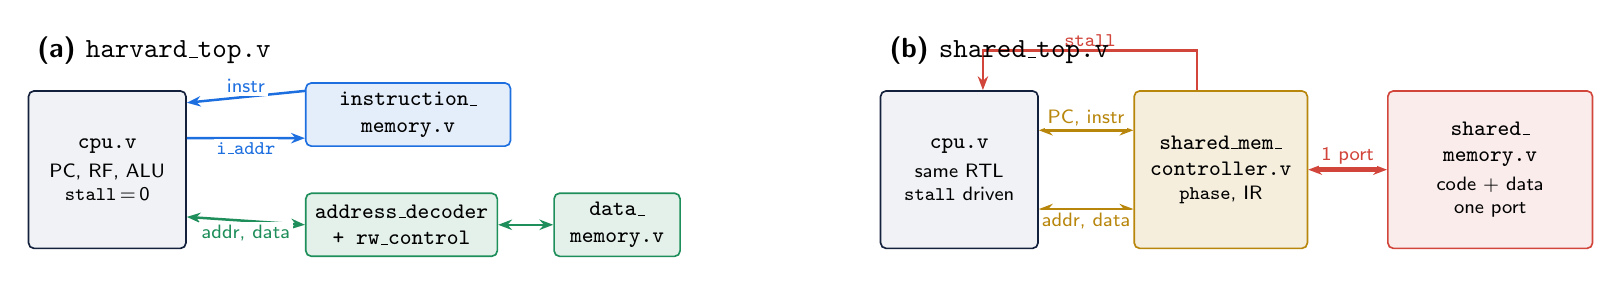
\begin{tikzpicture}[
  font=\sffamily\footnotesize, >={Stealth[length=5pt]},
  blk/.style={draw, rounded corners=2pt, align=center, line width=0.6pt, minimum height=8mm},
  cpu/.style={blk, fill=pnbg, draw=pnink, minimum width=20mm, minimum height=20mm},
  im/.style={blk, fill=pnblue!12, draw=pnblue, minimum width=26mm},
  dm/.style={blk, fill=pngreen!12, draw=pngreen, minimum width=22mm},
  sm/.style={blk, fill=pnred!10, draw=pnred, minimum width=26mm, minimum height=20mm},
  ct/.style={blk, fill=pnamber!14, draw=pnamber, minimum width=22mm, minimum height=20mm},
  lab/.style={font=\sffamily\scriptsize, fill=white, inner sep=1pt},
]
\node[cpu] (c1) {\texttt{cpu.v}\\[1pt]\scriptsize PC, RF, ALU\\[-1pt]\scriptsize \texttt{stall}\,=\,0};
\node[im, right=15mm of c1, yshift=7mm] (imem) {\texttt{instruction\_}\\\texttt{memory.v}};
\node[dm, right=15mm of c1, yshift=-7mm] (dec1) {\texttt{address\_decoder}\\\texttt{+ rw\_control}};
\node[dm, right=7mm of dec1, minimum width=16mm] (dmem) {\texttt{data\_}\\\texttt{memory.v}};
\draw[->, pnblue, line width=0.9pt] ($(c1.east)+(0,4mm)$) -- node[lab, below]{\texttt{i\_addr}} ($(imem.west)+(0,-3mm)$);
\draw[->, pnblue, line width=0.9pt] ($(imem.west)+(0,3mm)$) -- node[lab, above]{instr} ($(c1.east)+(0,8.5mm)$);
\draw[<->, pngreen, line width=0.9pt] ($(c1.east)+(0,-6mm)$) -- node[lab, below]{addr, data} (dec1.west);
\draw[<->, pngreen, line width=0.9pt] (dec1) -- (dmem);
\node[font=\sffamily\bfseries, anchor=south west] at ($(c1.north west)+(0,2mm)$) {(a) \texttt{harvard\_top.v}};

\node[cpu, right=88mm of c1] (c2) {\texttt{cpu.v}\\[1pt]\scriptsize same RTL\\[-1pt]\scriptsize \texttt{stall} driven};
\node[ct, right=12mm of c2] (ctl) {\texttt{shared\_mem\_}\\\texttt{controller.v}\\[-1pt]\scriptsize \texttt{phase}, IR};
\node[sm, right=10mm of ctl] (smem) {\texttt{shared\_}\\\texttt{memory.v}\\[1pt]\scriptsize code + data\\[-1pt]\scriptsize one port};
\draw[<->, pnamber, line width=0.9pt] ($(c2.east)+(0,5mm)$) -- node[lab, above]{PC, instr} ($(ctl.west)+(0,5mm)$);
\draw[<->, pnamber, line width=0.9pt] ($(c2.east)+(0,-5mm)$) -- node[lab, below]{addr, data} ($(ctl.west)+(0,-5mm)$);
\draw[->, pnred, line width=0.9pt] ($(ctl.north)+(-3mm,0)$) -- ++(0,5mm) -| node[lab, pos=0.25, above]{\texttt{stall}} ($(c2.north)+(3mm,0)$);
\draw[<->, pnred, line width=1.6pt] (ctl) -- node[lab, above]{1 port} (smem);
\node[font=\sffamily\bfseries, anchor=south west] at ($(c2.north west)+(0,2mm)$) {(b) \texttt{shared\_top.v}};
\end{tikzpicture}
\caption{The same \texttt{cpu.v} instance drives both top-level modules. (a) Harvard: independent
instruction (blue) and data (green) paths; the processor is never stalled. (b) Shared: the port
controller (amber) multiplexes one memory port between fetch and data access and stalls the
processor whenever both are required in the same cycle. The decoder, read/write control, and output
register of (a) are also present in (b) and omitted here for clarity.}
\label{fig:arch}
\end{figure*}

\subsection{Harvard System (\texttt{harvard\_top.v})}
The Harvard top level (\cref{fig:arch}a) wires the program counter directly to a $64\times16$
read-only instruction memory, and the data port through the decoder and read/write control to a
$64\times16$ data memory and the output register. \sig{stall} is tied to 0. Both memories are read
combinationally, so an instruction and its operand are both available within the cycle in which the
instruction is fetched, and the data memory is written on the rising clock edge when \sig{d_we} is
1. Instruction/data separation is enforced structurally, not by convention: the instruction memory
module exposes no write port at all.

\subsection{Shared-Memory System and the Port Controller}
\label{sec:controller}
The shared top level stores code (\texttt{0x00}--\texttt{0x0F}) and data
(\texttt{0x10}--\texttt{0x2F}) in one $64\times16$ array with exactly one address/data port. The
controller (\cref{alg:ctrl,fig:fsm}) arbitrates that port with a one-bit state \sig{phase} and a
16-bit latch \sig{IR}. In the fetch phase the port is addressed by the program counter. If the word
just read is a \textsc{load} or \textsc{store}, the controller raises \sig{stall}, latches the word
into \sig{IR}, and moves to the data phase; otherwise the instruction is complete. In the data
phase the port is addressed by the data address, the processor executes from \sig{IR}, writes are
enabled, and the controller returns to the fetch phase.

\begin{algorithm}[t]
\caption{Port controller, one clock cycle (\texttt{rtl/shared\_mem\_controller.v})}
\label{alg:ctrl}
\footnotesize
\begin{algorithmic}[1]
\If{$\mathit{phase}=0$} \Comment{fetch phase}
  \State $\mathit{mem\_addr} \gets \mathit{PC}$;\; $\mathit{instr} \gets M[\mathit{PC}]$
  \If{$\mathrm{op}(M[\mathit{PC}]) \in \{\textsc{load},\textsc{store}\}$}
    \State $\mathit{stall}\gets1$;\; $\mathit{IR}\gets M[\mathit{PC}]$;\; $\mathit{phase}\gets1$
  \Else
    \State $\mathit{stall}\gets0$ \Comment{instruction completes}
  \EndIf
\Else \Comment{data phase}
  \State $\mathit{mem\_addr}\gets\mathit{d\_addr}$;\; $\mathit{instr}\gets\mathit{IR}$; writes enabled
  \State $\mathit{stall}\gets0$;\; $\mathit{phase}\gets0$ \Comment{access completes}
\EndIf
\end{algorithmic}
\end{algorithm}

\begin{figure}[t]
\centering
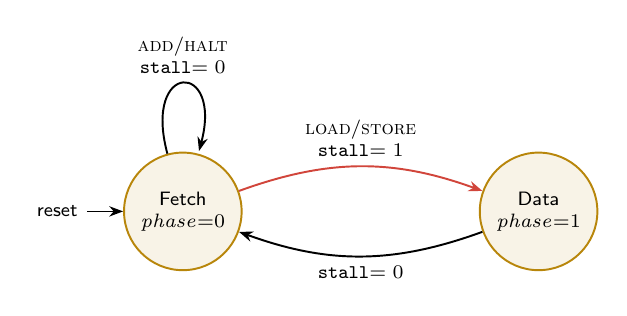
\begin{tikzpicture}[font=\sffamily\scriptsize, >={Stealth[length=5pt]}, node distance=30mm,
  every state/.style={draw=pnamber, fill=pnamber!10, line width=0.7pt, minimum size=14mm, align=center}]
\node[state, initial, initial text=reset] (F) {Fetch\\$\mathit{phase}{=}0$};
\node[state, right=of F] (D) {Data\\$\mathit{phase}{=}1$};
\path[->, line width=0.7pt]
 (F) edge[loop above] node[align=center]{\textsc{add}/\textsc{halt}\\ \texttt{stall}$=0$} (F)
 (F) edge[bend left=20, draw=pnred] node[above, align=center]{\textsc{load}/\textsc{store}\\ \texttt{stall}$=1$} (D)
 (D) edge[bend left=20] node[below, align=center]{\texttt{stall}$=0$} (F);
\end{tikzpicture}
\caption{Controller state machine. \texttt{stall} is a Mealy output: it depends on the state
\emph{and} on the opcode of the word just read from the port.}
\label{fig:fsm}
\end{figure}

\textit{Avoiding a combinational loop.} The project's design notes record that the first design
stalled whenever the processor itself requested a data access, i.e.\ on $\mathit{d\_re} \vee
\mathit{d\_we}$. But \cref{eq:run} forces $\mathit{d\_we}=0$ while $\mathit{stall}=1$, so under that
rule \sig{stall} would depend combinationally on \sig{d_we}, and \sig{d_we} on \sig{stall}: for a
\textsc{store}, raising \sig{stall} would clear \sig{d_we}, which would clear \sig{stall}, with no
stable fixed point. The controller instead decodes the opcode bits of the fetched word directly
(\cref{lst:ctrl}), a signal that depends only on the memory's read data and the registered
\sig{phase}, neither of which depends on \sig{stall} combinationally. The externally observable
behaviour is unchanged; only the signal the decision is taken from is different.

\begin{lstlisting}[caption={Port arbitration, verbatim from \texttt{rtl/shared\_mem\_controller.v}.},label={lst:ctrl},float=t]
wire is_mem_op = (fetched_op == 4'd2) ||
                 (fetched_op == 4'd3);
assign stall    = ~phase & is_mem_op;
assign instr    = phase ? IR     : mem_rdata;
assign mem_addr = phase ? d_addr : pc;
assign mem_we   = phase & data_we;
\end{lstlisting}

\subsection{Analytical Cycle Model}
\label{sec:model}
\begin{definition}
A program executes a dynamic sequence of $N$ instructions, including the terminating
\textsc{halt}, of which $\NLS$ are \textsc{load} or \textsc{store}. Its \emph{data-access fraction}
is $f = \NLS/N \in [0,1)$. The \emph{cycle count} $T$ of a system is the number of rising clock
edges from reset release until \sig{halted} is asserted, inclusive of the cycle in which
\textsc{halt} executes.
\end{definition}

\begin{proposition}\label{prop:cycles}
For every program accepted by this instruction set, $\Tharv = N$ and $\Tshr = N + \NLS$.
\end{proposition}
\begin{proof}
\emph{Harvard.} \sig{stall} is the constant 0, so by \cref{eq:run} every fetched instruction
completes, architecturally, in the same cycle in which it is fetched; hence $\Tharv = N$.
\emph{Shared.} Reset drives \sig{phase} to 0, and both transitions of \cref{fig:fsm} return to
$\mathit{phase}=0$, so every instruction is first presented in the fetch phase. An \textsc{add} or
\textsc{halt} completes in that same cycle. A \textsc{load} or \textsc{store} instead raises
\sig{stall}, which by \cref{eq:run} gives that cycle no architectural effect; on the following
cycle $\mathit{phase}=1$ and $\mathit{stall}=0$, the instruction completes from \sig{IR}, and
\sig{phase} returns to 0. Every memory instruction therefore costs exactly two cycles and every
other instruction costs one, so $\Tshr = (N - \NLS)\cdot 1 + \NLS \cdot 2 = N + \NLS$.
\end{proof}

\begin{corollary}\label{cor:cpi}
$\mathrm{CPI}_{\mathrm{H}} = 1$, $\mathrm{CPI}_{\mathrm{S}} = 1 + f$, and the Harvard speedup over the
shared system is $S = \Tshr/\Tharv = 1 + f$.
\end{corollary}

\textit{Port-demand bound.} Each instruction requires exactly one fetch and, with probability $f$,
one data access, so a workload demands $1+f$ memory accesses per instruction on average. A
single port can supply at most one access per cycle, which bounds the shared system's throughput
from above:
\begin{equation}
  \mathrm{IPC}_{\mathrm{S}} \le \frac{1}{1+f}, \qquad \mathrm{IPC}_{\mathrm{H}} = 1 .
  \label{eq:ipc}
\end{equation}
The controller in \cref{sec:controller} meets this bound with equality, because the single port is
busy on every cycle: once in the fetch phase and, for every memory instruction, once more in the
data phase. \Cref{fig:ipc} plots \cref{eq:ipc} together with the three measured workloads.

\begin{figure}[t]
\centering
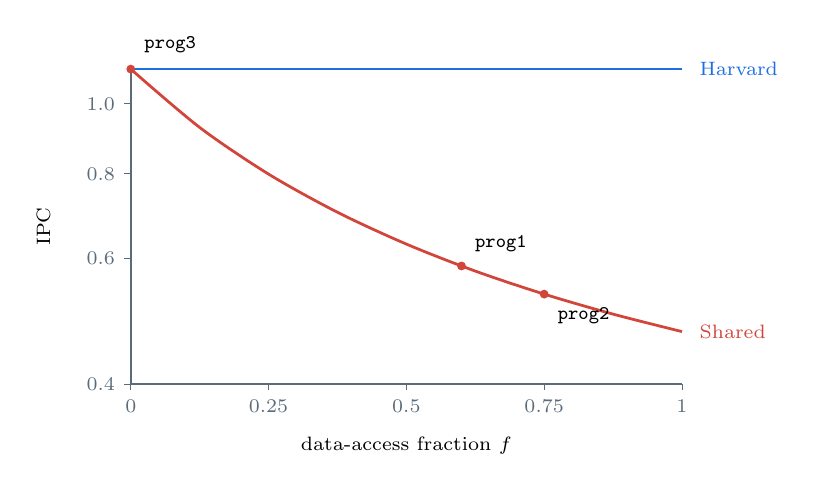
\begin{tikzpicture}
\begin{scope}
  \def\axw{7.0} \def\axh{4.0}
  \draw[pnslate, line width=0.6pt] (0,0) -- (0,\axh);
  \draw[pnslate, line width=0.6pt] (0,0) -- (\axw,0);
  \foreach \x/\lab in {0/0,1.75/0.25,3.5/0.5,5.25/0.75,7/1}
    \draw[pnslate, line width=0.3pt] (\x,0) -- (\x,-0.08) node[below, font=\scriptsize] {\lab};
  \foreach \y/\lab in {0/0.4,1.6/0.6,2.67/0.8,3.56/1.0}
    \draw[pnslate, line width=0.3pt] (0,\y) -- (-0.08,\y) node[left, font=\scriptsize] {\lab};
  \node[rotate=90, font=\scriptsize, anchor=south] at (-0.9,\axh/2) {IPC};
  \node[font=\scriptsize, anchor=north] at (\axw/2,-0.55) {data-access fraction $f$};
  % Harvard: IPC = 1 (flat line), mapped y = (1-0.4)/0.6*axh
  \draw[pnblue, line width=1pt] (0,{(1-0.4)/0.6*\axh}) -- (\axw,{(1-0.4)/0.6*\axh});
  % Shared: IPC = 1/(1+f), f in [0,1], sampled
  \draw[pnred, line width=1pt]
    plot[smooth] coordinates {
      (0,{(1-0.4)/0.6*\axh})
      (0.875,{(1/1.125-0.4)/0.6*\axh})
      (1.75,{(1/1.25-0.4)/0.6*\axh})
      (2.625,{(1/1.375-0.4)/0.6*\axh})
      (3.5,{(1/1.5-0.4)/0.6*\axh})
      (4.375,{(1/1.625-0.4)/0.6*\axh})
      (5.25,{(1/1.75-0.4)/0.6*\axh})
      (6.125,{(1/1.875-0.4)/0.6*\axh})
      (7,{(1/2-0.4)/0.6*\axh})
    };
  % Measured markers: prog1 f=0.6, prog2 f=0.75, prog3 f=0
  \fill[pnred] ({0.6*7},{(1/1.6-0.4)/0.6*\axh}) circle (1.6pt);
  \node[font=\scriptsize, anchor=south west] at ({0.6*7+0.05},{(1/1.6-0.4)/0.6*\axh+0.05}) {\texttt{prog1}};
  \fill[pnred] ({0.75*7},{(1/1.75-0.4)/0.6*\axh}) circle (1.6pt);
  \node[font=\scriptsize, anchor=north west] at ({0.75*7+0.05},{(1/1.75-0.4)/0.6*\axh-0.05}) {\texttt{prog2}};
  \fill[pnred] (0,{(1-0.4)/0.6*\axh}) circle (1.6pt);
  \node[font=\scriptsize, anchor=south west] at (0.05,{(1-0.4)/0.6*\axh+0.08}) {\texttt{prog3}};
  \node[pnblue, font=\scriptsize, anchor=west] at (7.1,{(1-0.4)/0.6*\axh}) {Harvard};
  \node[pnred, font=\scriptsize, anchor=west] at (7.1,{(1/2-0.4)/0.6*\axh}) {Shared};
\end{scope}
\end{tikzpicture}
\caption{Throughput bound \cref{eq:ipc} as a function of the data-access fraction $f$. Markers are
the three measured workloads (\cref{tab:results}); each sits exactly on the shared-system curve,
since the controller meets the bound with equality.}
\label{fig:ipc}
\end{figure}

\subsection{Experimental Setup}
\label{sec:method}
\textit{Implementation.} The design comprises twelve synthesizable Verilog-2001 modules with
synchronous, active-high reset and no simulation-only constructs in the RTL itself: six are shared
by both systems (\texttt{program\_counter}, \texttt{register\_file}, \texttt{cpu},
\texttt{address\_decoder}, \texttt{rw\_control}, \texttt{io\_reg}); the Harvard system adds
\texttt{instruction\_memory}, \texttt{data\_memory}, and \texttt{harvard\_top}; the shared system
adds \texttt{shared\_memory}, \texttt{shared\_mem\_controller}, and \texttt{shared\_top}. For this
paper we simulated the design with Icarus~Verilog~13.0 (\texttt{-g2001 -Wall}) rather than relying
solely on the authors' own prior runs, so every number reported in \cref{sec:results} was
reproduced independently while writing this report.

\textit{Workloads.} Three hand-encoded programs (\cref{tab:workloads}) exercise complementary
behaviour. \texttt{prog1} is the reference workload, with three memory operations out of five
instructions ($f=0.6$). \texttt{prog2} exercises address decoding, including a store to the output
register and a store to an unmapped address, with three memory operations out of four instructions
($f=0.75$). \texttt{prog3} performs three additions and no memory operation at all ($f=0$); with no
\textsc{load} instruction in the set and \sig{R0} fixed at zero, it can only ever add zeros to
zeros, so it serves purely as a control case for which \cref{prop:cycles} predicts identical cycle
counts on both systems.

\begin{table}[t]
\centering
\caption{Workloads and Checked Properties (\texttt{programs/})}
\label{tab:workloads}
\footnotesize
\begin{tabularx}{\columnwidth}{@{}l >{\ttfamily}l X@{}}
\toprule
Prog. & \normalfont Machine code & Checked properties \\
\midrule
\texttt{prog1} & 2210 2411 1650 3620 0000 & R1\,=\,5, R2\,=\,7, R3\,=\,12, $M[\texttt{0x20}]$\,=\,12 \\
\texttt{prog2} & 2210 323F 3230 0000 & \sig{io_out}\,=\,5; \sig{addr_err} raised; $M[\texttt{0x30}], M[\texttt{0x3F}]$ unchanged \\
\texttt{prog3} & 1200 1448 1690 0000 & R1\,=\,R2\,=\,R3\,=\,0 (no memory access) \\
\bottomrule
\end{tabularx}
\end{table}

\textit{Verification.} Each system has a self-checking testbench (\texttt{tb\_harvard.v},
\texttt{tb\_shared.v}) that releases reset, runs until \sig{halted} or 200 cycles elapse, compares
the final architectural state and the cycle count against expected values, and prints
\textsc{pass} or \textsc{fail} with the exact mismatch. The Makefile's \texttt{compare} target runs
all six Harvard/shared $\times$ three-program configurations and tabulates the results; a
testbench parameter, \sig{PROG_NUM}, selects the program and data file by a ternary chain over
three equal-length file names so that \sig{\$readmemh} always receives an intact string. Because
every memory is 64 words but the five-to-six-word programs are shorter,
\sig{\$readmemh} emits a benign ``not enough words'' warning on every run; it is harmless, since
every memory is zero-filled (encoding \textsc{halt}) before the program is loaded, and the
Makefile filters the warning out of its own output.

\textit{Fault injection.} To confirm that a passing result reflects correct behaviour rather than a
vacuous check, the project's design notes record a direct test of the testbenches themselves:
replacing the adder in \texttt{cpu.v} with a subtractor. On \texttt{prog1}, the \texttt{check} task
then reports a mismatch on \textsc{r3} (the two's-complement wraparound of $5-7$) instead of
passing, confirming that the comparison in \cref{tab:workloads} is a genuine functional check.

\subsection{What the Three Workloads Do Not Show}
The project's own design notes flag a limitation of the test suite explicitly, and we preserve it
here rather than letting the results in \cref{sec:results} overstate what was demonstrated: no test
program stores into the program region (\texttt{0x00}--\texttt{0x0F}) of the shared memory, so the
claim that ``a store could overwrite the program in the shared system, but not in the Harvard
system'' is argued from the RTL (the Harvard instruction memory has no write port; the shared
memory's single write port has no address restriction) rather than demonstrated by a failing-then-
passing test. It is noted here as a talking point and as a concrete direction for a fourth workload,
not as a validated result.

% =============================================================================
\section{Results and Discussion}
\label{sec:results}
% =============================================================================

\subsection{Cycle Counts}
All six configurations pass under the Icarus~Verilog~13.0 run performed for this paper, and every
measured cycle count equals the prediction of \cref{prop:cycles} (\cref{tab:results,fig:bars}). The
gap between the two systems equals $\NLS$ for every workload and is exactly zero for the control
workload, as predicted.

\begin{table}[t]
\centering
\caption{Measured Cycle Counts Versus the Model}
\label{tab:results}
\footnotesize
\begin{tabular}{@{}l c c c c c c@{}}
\toprule
Prog. & $N$ & $\NLS$ & $f$ & $\Tharv$ & $\Tshr$ (meas./model) & $S$ \\
\midrule
\texttt{prog1} & 5 & 3 & 0.60 & 5 & 8 / 8 & 1.60 \\
\texttt{prog2} & 4 & 3 & 0.75 & 4 & 7 / 7 & 1.75 \\
\texttt{prog3} & 4 & 0 & 0.00 & 4 & 4 / 4 & 1.00 \\
\bottomrule
\end{tabular}
\end{table}

\begin{figure}[t]
\centering
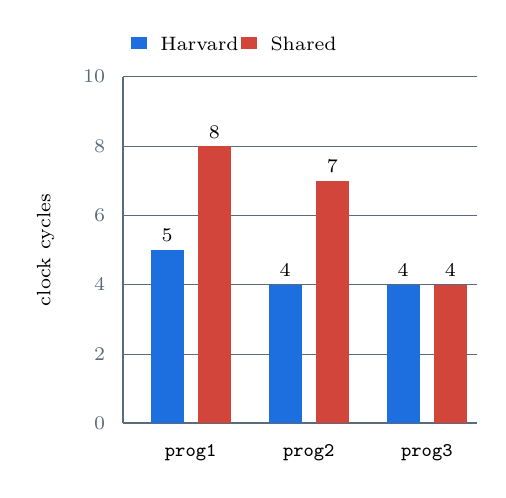
\begin{tikzpicture}
  \def\axh{4.4} \def\barw{0.42} \def\gap{0.18} \def\groupw{1.5}
  \draw[pnslate, line width=0.6pt] (0,0) -- (3*\groupw,0);
  \draw[pnslate, line width=0.6pt] (0,0) -- (0,\axh);
  \foreach \y in {0,2,4,6,8,10}
    \draw[pnslate, line width=0.2pt] (0,{\y/10*\axh}) -- (3*\groupw,{\y/10*\axh})
      node[left, font=\scriptsize, pos=0, xshift=-3pt] {\y};
  \foreach \i/\name/\h in {0/prog1/5,1/prog2/4,2/prog3/4}{
    \fill[pnblue] ({\i*\groupw+0.35},0) rectangle ({\i*\groupw+0.35+\barw},{\h/10*\axh});
    \node[font=\scriptsize] at ({\i*\groupw+0.35+\barw/2},{\h/10*\axh+0.18}) {\h};
  }
  \foreach \i/\name/\h in {0/prog1/8,1/prog2/7,2/prog3/4}{
    \fill[pnred] ({\i*\groupw+0.35+\barw+\gap},0) rectangle ({\i*\groupw+0.35+2*\barw+\gap},{\h/10*\axh});
    \node[font=\scriptsize] at ({\i*\groupw+0.35+1.5*\barw+\gap},{\h/10*\axh+0.18}) {\h};
  }
  \foreach \i/\name in {0/prog1,1/prog2,2/prog3}
    \node[font=\ttfamily\scriptsize, anchor=north] at ({\i*\groupw+0.35+\barw+\gap/2},-0.15) {\name};
  \node[rotate=90, font=\scriptsize, anchor=south] at (-0.75,\axh/2) {clock cycles};
  \fill[pnblue] (0.1,\axh+0.35) rectangle (0.3,\axh+0.5); \node[font=\scriptsize, anchor=west] at (0.35,\axh+0.42) {Harvard};
  \fill[pnred] (1.5,\axh+0.35) rectangle (1.7,\axh+0.5); \node[font=\scriptsize, anchor=west] at (1.75,\axh+0.42) {Shared};
\end{tikzpicture}
\caption{Cycles to completion for each workload, measured in this paper's own simulation run.}
\label{fig:bars}
\end{figure}

\subsection{Timing Behaviour, Verified Cycle by Cycle}
To check the mechanism in \cref{sec:controller}, not only its final cycle count, we instrumented a
scratch copy of \texttt{shared\_top.v}'s instantiation to print \sig{phase}, \sig{stall}, and
\sig{mem_addr} on every clock edge while running \texttt{prog1}, and did the same for
\texttt{i\_addr}/\texttt{d\_addr} in the Harvard system. \Cref{tab:trace} reports the result. In the
Harvard system, \texttt{i\_addr} and \texttt{d\_addr} are both driven to a live address in cycles
0, 1, and 3 --- precisely the cycles that execute \textsc{load} or \textsc{store} --- confirming
that fetch and data access genuinely overlap on every memory instruction rather than merely by
assumption. In the shared system, every memory instruction's fetch cycle has \sig{stall}\,=\,1 and
\sig{mem_addr} equal to the program counter, immediately followed by a cycle with \sig{stall}\,=\,0
and \sig{mem_addr} equal to the data address; the \textsc{add} at \texttt{0x02} and the
\textsc{halt} at \texttt{0x04} each occupy a single fetch-phase cycle with no stall. This is the
address-by-address confirmation of the state machine in \cref{fig:fsm}, not merely of its net
cycle count.

\begin{table}[t]
\centering
\caption{Verified Cycle-by-Cycle Trace of \texttt{prog1}, by Instruction}
\label{tab:trace}
\footnotesize
\begin{tabularx}{\columnwidth}{@{}l c l c X@{}}
\toprule
Instr.\ (PC) & \multicolumn{2}{c}{Harvard} & \multicolumn{2}{c}{Shared} \\
 & cyc. & \texttt{i\_/d\_addr} & cyc. & \texttt{mem\_addr} trace (\texttt{stall}) \\
\midrule
\textsc{load} (00) & 0 & \texttt{00}/\texttt{10} & 0--1 & \texttt{00}(1) $\to$ \texttt{10}(0) \\
\textsc{load} (01) & 1 & \texttt{01}/\texttt{11} & 2--3 & \texttt{01}(1) $\to$ \texttt{11}(0) \\
\textsc{add} (02) & 2 & \texttt{02}/--- & 4 & \texttt{02}(0) \\
\textsc{store} (03) & 3 & \texttt{03}/\texttt{20} & 5--6 & \texttt{03}(1) $\to$ \texttt{20}(0, write) \\
\textsc{halt} (04) & 4 & \texttt{04}/--- & 7 & \texttt{04}(0) \\
\bottomrule
\end{tabularx}

\vspace{2pt}
\footnotesize\textit{Harvard finishes in 5 cycles (0--4), one per instruction. The shared system
finishes in 8 cycles (0--7), tracing the single-port address sequence \texttt{00, 10, 01, 11, 02,
03, 20, 04}: every \textsc{load}/\textsc{store} costs two port cycles (fetch, marked
\texttt{stall}\,=\,1, then data) while \textsc{add} and \textsc{halt} cost one. The 3-cycle gap
matches the 3 \textsc{load}/\textsc{store} instructions in \texttt{prog1} exactly.}
\end{table}

\subsection{Memory-Mapped I/O and Address Decoding}
\texttt{prog2} exercises both outcomes of the address decoder. Its store to \texttt{0x3F} reaches
the output register, \sig{io_out}, in both systems. Its store to the unmapped address \texttt{0x30}
raises \sig{addr_err} for exactly the one cycle in which that store's data access occurs and is
otherwise silently discarded: \cref{tab:results}'s checks confirm \texttt{0x30} and \texttt{0x3F}
of the data memory (Harvard) are unchanged, i.e.\ the unmapped write never reached memory and the
I/O write never reached memory either. \sig{addr_err} is deasserted in every other cycle of this
run, including the cycle executing the earlier \textsc{load}, because of the access qualifier
described in \cref{sec:design}.

\subsection{Interpretation}
Because the processor, the three workloads, and the address map are identical between the two
systems, the measured difference in cycle count can be attributed only to the memory organization.
The control workload, \texttt{prog3}, confirms this directly by producing identical cycle counts on
both systems. The model in \cref{sec:model} is exact for this design because the controller adds
precisely one cycle for every memory instruction and none for any other instruction; equivalently,
the shared system's single port is busy in every cycle it runs, so it operates exactly at the bound
of \cref{eq:ipc} rather than merely below it.

The same resource conflict recurs in pipelined processors whenever an instruction fetch and a data
access land in the same pipeline stage in the same cycle, which is the practical reason production
processors place separate level-one instruction and data caches in front of one shared main memory.
The measurements here quantify, for the smallest machine in which the effect is visible at all, what
that separation is worth: a throughput factor of $1+f$, roughly 60--75\% for the two data-touching
workloads measured. Because caches, prefetching, and pipelining all change this balance in ways the
present model does not capture, the figure should be read as the benefit of separation in a
non-pipelined, cache-free machine, not as a prediction for a real CPU.

\subsection{README's Own Waveform Checklist, Mapped to This Paper}
The project README lists specific signals and cycles for a reader to inspect in GTKWave as a
sanity check on the design. \Cref{tab:objectives} maps each of those checkpoints to where it is now
backed by a number in this paper, rather than only by a visual inspection.

\begin{table}[t]
\centering
\caption{README's GTKWave Checklist, Mapped to This Paper's Evidence}
\label{tab:objectives}
\footnotesize
\begin{tabularx}{\columnwidth}{@{}>{\raggedright\arraybackslash}p{0.40\columnwidth} X@{}}
\toprule
README checkpoint & Evidence in this paper \\
\midrule
Harvard, \texttt{prog1}: \texttt{i\_addr} and \texttt{d\_addr} both active in the same cycle & \cref{tab:trace}, cycles 0, 1, 3 \\
Shared, \texttt{prog1}: \texttt{mem\_addr}\,=\,PC with \texttt{stall}\,=\,1, then \texttt{mem\_addr}\,=\,data address next cycle & \cref{tab:trace}, address pairs (\texttt{00},\texttt{10}), (\texttt{01},\texttt{11}), (\texttt{03},\texttt{20}) \\
\texttt{make compare} table (LOAD/STORE, Harvard/Shared cycles, Extra) & \cref{tab:results}, columns $\NLS$, $\Tharv$, $\Tshr$ \\
\texttt{addr\_err} only on a real unmapped access & \cref{sec:design} access qualifier; \cref{tab:results} \texttt{prog2} checks \\
\bottomrule
\end{tabularx}
\end{table}

\subsection{Threats to Validity}
\textit{Idealized memories.} Both memories are modelled as combinational-read arrays with no access
latency; a synchronous SRAM or a DRAM would add latency to both systems, but under this model's
assumptions the \emph{relative} cost of port contention would be unaffected. \textit{Processor
model.} The result applies to a non-pipelined, single-cycle processor; in a pipeline the cost would
also depend on scheduling, forwarding, and pipeline depth. \textit{Workloads.} Three short,
hand-encoded programs exercise every datapath and control path exactly once each but are not
representative of application-level instruction mixes; without an immediate or load-constant
instruction, \texttt{prog3} can only ever add zeros. \textit{Scope of testing.} As noted in
\cref{sec:method}, no test exercises a store into the shared system's program region, so the
instruction/data-separation argument for that case rests on inspection of the RTL rather than on a
test. \textit{Implementation.} The RTL follows synthesizable Verilog-2001 conventions but was
evaluated only in simulation; clock frequency and silicon area were not measured.

% =============================================================================
\section{Conclusion}
\label{sec:conclusion}
% =============================================================================
This project built one single-cycle, four-instruction processor and attached it, unmodified, to a
Harvard memory system and to a single-ported shared-memory system whose controller resolves the
resulting structural hazard by stalling on the opcode of the word it has just fetched. Analysis and
simulation agree, and for this paper we additionally re-verified the mechanism cycle by cycle rather
than relying only on the repository's own prior test runs. The Harvard organization sustains one
instruction per cycle because every load and store performs its fetch and its data access in the
same cycle; the shared organization needs exactly one extra cycle per load or store,
$\Tshr = \Tharv + \NLS$, giving $\mathrm{CPI} = 1+f$ and a throughput bound
$\mathrm{IPC}_{\mathrm{S}} \le 1/(1+f)$ that the design meets with equality. Natural extensions
noted by the team include a fourth workload that stores into the shared program region to make the
code-integrity argument a tested result rather than an inspection, branch and immediate
instructions to allow loop-based programs, a synchronous memory model with realistic latency, and a
pipelined version of the processor to see how the same hazard interacts with forwarding.

% =============================================================================
\section*{Author Contributions}
% =============================================================================
\noindent{\footnotesize
\begin{tabularx}{\columnwidth}{@{}l X@{}}
\toprule
Author & Contribution (modules, per \texttt{README.md}) \\
\midrule
Aryan Vibhuti & Register file and program counter: \texttt{register\_file.v}, \texttt{program\_counter.v} \\
Saswataduity Bhuin & Processor: instruction decode, control, address generation, and stall gating: \texttt{cpu.v} \\
Debasish Karan & Address decoding, read/write control, and the memory-mapped output register: \texttt{address\_decoder.v}, \texttt{rw\_control.v}, \texttt{io\_reg.v} \\
Aryu Rao & Harvard memories and integration, Harvard testbench, test programs, build flow, and project documentation: \texttt{instruction\_memory.v}, \texttt{data\_memory.v}, \texttt{harvard\_top.v}, \texttt{tb\_harvard.v}, \texttt{programs/}, \texttt{Makefile}, \texttt{README.md}, \texttt{docs/decisions.md} \\
Sayan Bhattacharya & Shared memory, port controller, shared system integration, and shared testbench: \texttt{shared\_memory.v}, \texttt{shared\_mem\_controller.v}, \texttt{shared\_top.v}, \texttt{tb\_shared.v} \\
\bottomrule
\end{tabularx}}

\vspace{4pt}\noindent All authors contributed to the analysis of the results and approved the final
manuscript. The independent re-verification and the cycle-by-cycle trace reported in
\cref{sec:results} were performed while drafting this paper, using the simulation toolchain and
test programs the team had already committed to the repository.

\end{document}
